%%%%%%%%%%%%%%%%%%%%%%%%%%%%%%%%%%%%%%%%%%%%%%%%%%%%%%%%%%%%%%%%%%%
%                                                                 %
%  GEANT manual in LaTeX form                              %
%                                                                 %
%  Michel Goossens (for translation into LaTeX)                   %
%  Version 1.00                                                   %
%  Last Mod. Jan 24 1991  1300   MG + IB                          %
%                                                                 %
%%%%%%%%%%%%%%%%%%%%%%%%%%%%%%%%%%%%%%%%%%%%%%%%%%%%%%%%%%%%%%%%%%%
\Origin{R.Brun}
\Submitted{01.11.78}     \Revised{14.12.93}
\Version{Geant 3.16}     \Routid{GEOM299}
\Makehead{The rotation matrix data structure JROTM}
 
\begin{figure}[hbt]
     \centering
     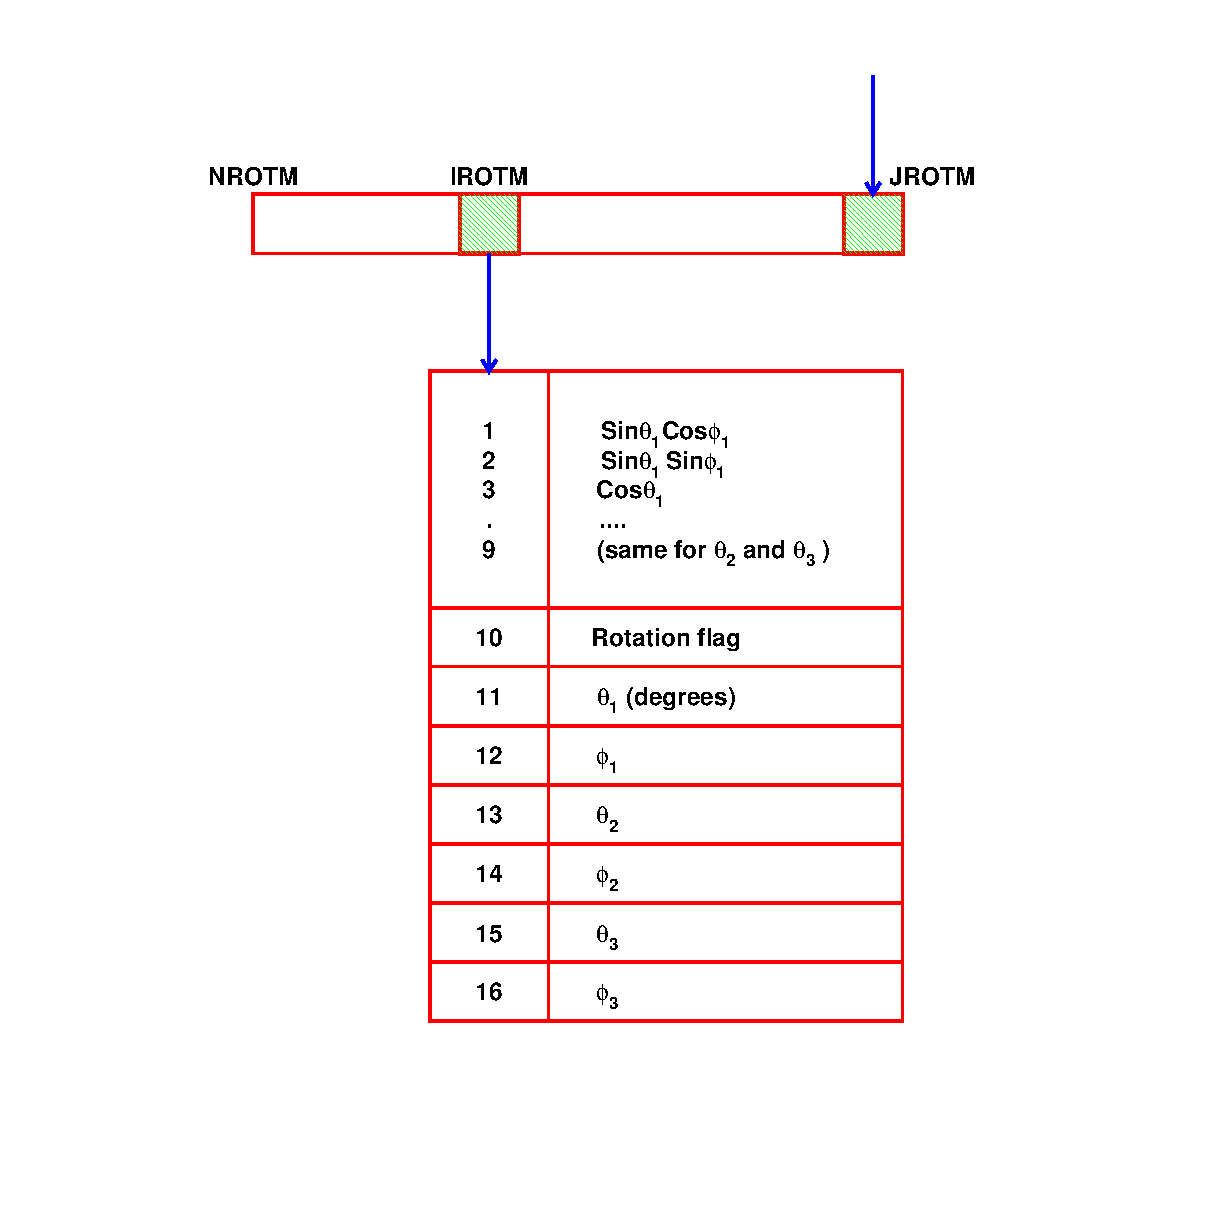
\epsfig{file=eps/geom299-1.eps,width=14cm}
     \caption{Layout of the {\tt JROTM} data structure}
     \label{fg:geom299-1}
\end{figure}

{\tt JR = LQ(JROTM-IROTM)} is the
pointer to the bank of the rotation matrix {\tt IROTM};
 
The rotation flag is computed by \Rind{GSROTM} to 
recognise simple rotation configurations. In particular it
is set to 0 for the unit matrix. 
